\documentclass[12pt]{article}
\usepackage{url, graphicx, epstopdf, amsmath, esint}
\usepackage{physics}

% page layout
\setlength{\topmargin}{-0.25in}
\setlength{\textheight}{9.5in}
\setlength{\headheight}{0in}
\setlength{\headsep}{0in}
\setlength{\parindent}{1.1\baselineskip}
\addtolength{\oddsidemargin}{-0.75in}
\setlength{\marginparwidth}{2in}

% problem formatting
\newcommand{\problemname}{Problem}
\newcounter{problem}
\newcommand{\startproblem}{\paragraph{Problem~\theproblem:}\refstepcounter{problem}}

% words
\newcommand{\foreign}[1]{\textsl{#1}}
\newcommand{\vs}{\foreign{vs}}

% math
\renewcommand{\vec}[1]{\boldsymbol{#1}}
% \newcommand{\dd}{\mathrm{d}} % PROVIDED IN physics PACKAGE
\newcommand{\e}{\mathrm{e}}
% \newcommand{\cross}{\times} % PROVIDED IN physics PACKAGE
% \newcommand{\curl}{\vec{\nabla}\times} % PROVIDED IN physics PACKAGE

% primary units
\newcommand{\rad}{\mathrm{rad}}
\newcommand{\kg}{\mathrm{kg}}
\newcommand{\m}{\mathrm{m}}
\newcommand{\s}{\mathrm{s}}
\newcommand{\A}{\mathrm{A}}

% secondary units
\renewcommand{\deg}{\mathrm{deg}}
\newcommand{\km}{\mathrm{km}}
\newcommand{\cm}{\mathrm{cm}}
\newcommand{\mm}{\mathrm{mm}}
\newcommand{\mum}{\mathrm{\mu m}}
\newcommand{\nm}{\mathrm{nm}}
\newcommand{\ft}{\mathrm{ft}}
\newcommand{\mi}{\mathrm{mi}}
\newcommand{\AU}{\mathrm{AU}}
\newcommand{\ns}{\mathrm{ns}}
\newcommand{\h}{\mathrm{h}}
\newcommand{\yr}{\mathrm{yr}}
\newcommand{\N}{\mathrm{N}}
\newcommand{\J}{\mathrm{J}}
\newcommand{\eV}{\mathrm{eV}}
\newcommand{\MeV}{\mathrm{MeV}}
\newcommand{\W}{\mathrm{W}}
\newcommand{\Pa}{\mathrm{Pa}}
\newcommand{\C}{\mathrm{C}}
\newcommand{\V}{\mathrm{V}}
\newcommand{\ohm}{\mathrm{\Omega}}
\newcommand{\muF}{\mathrm{\mu F}}
\newcommand{\Hz}{\mathrm{Hz}}
\newcommand{\GHz}{\mathrm{GHz}}

% derived units
\newcommand{\mps}{\m\,\s^{-1}}
\newcommand{\mph}{\mi\,\h^{-1}}
\newcommand{\mpss}{\m\,\s^{-2}}
\newcommand{\radps}{\rad\,\s^{-1}}

% random stuff
\sloppy\sloppypar\raggedbottom\frenchspacing\thispagestyle{empty}

\begin{document}

\section*{NYU Physics 2---Problem Set 8}

Due Thursday 2022 April 7 by 12:30\,pm on Brightspace.

\startproblem%
Imagine that you have a block of conductor moving at velocity
$\vec{v}$ in the $x$-direction in a magnetic field $\vec{B}$ that is
constant and pointing in the $z$-direction. The charges will rearrange
in the conductor. The positive charges will get pushed in one
direction and the negative in the other.
The charges will move until there is no net force on any
charge inside the conductor.
That means that the conductor will
contain an internal electric field that counteracts the magnetic
forces on the charges.
That is, the electric field will be zero in the conductor \emph{in the conductor's rest frame} but not in general.
What is the direction and magnitude of this
electric field inside the conductor?

\textsl{Bonus special-relativity part (not for credit):} If you switch
into the rest frame of the block, then it is not moving, and there
must be no magnetic forces. So what must be the external $\vec{E}$ and
$\vec{B}$ fields in this frame?

\textsl{Bonus weirder relativity part (not for credit):} What do you
think happens in a stationary but \emph{rotating} (spinning) conductor in a magnetic
field?

\startproblem%
Compute the mutual
inductance between a solenoid of length $h$ and radius $a\ll h$ and
$N$ turns of wire and a single loop of radius $R>a$ (but $R\ll h$
still) surrounding the solenoid. Assume that the magnetic field is
strong inside the solenoid and essentially zero outside the solenoid,
so that you can make a definite (approximate) calculation. Your
calculation will be exact in the limit that $h$ is extremely large.

\startproblem%
Consider this circuit.
When the switch is open, the current is zero. If the switch is closed
at time $t=0$, what is the differential equation that governs the
current as a function of time? And what is its solution? That is,
what is the current $I(t)$?

\textsl{Hint:} The solution will involve $\exp(-\alpha t)$ for some
$\alpha$, and as $t\rightarrow\infty$, you will get $I(t)\rightarrow
V/R$. Why?
\marginpar{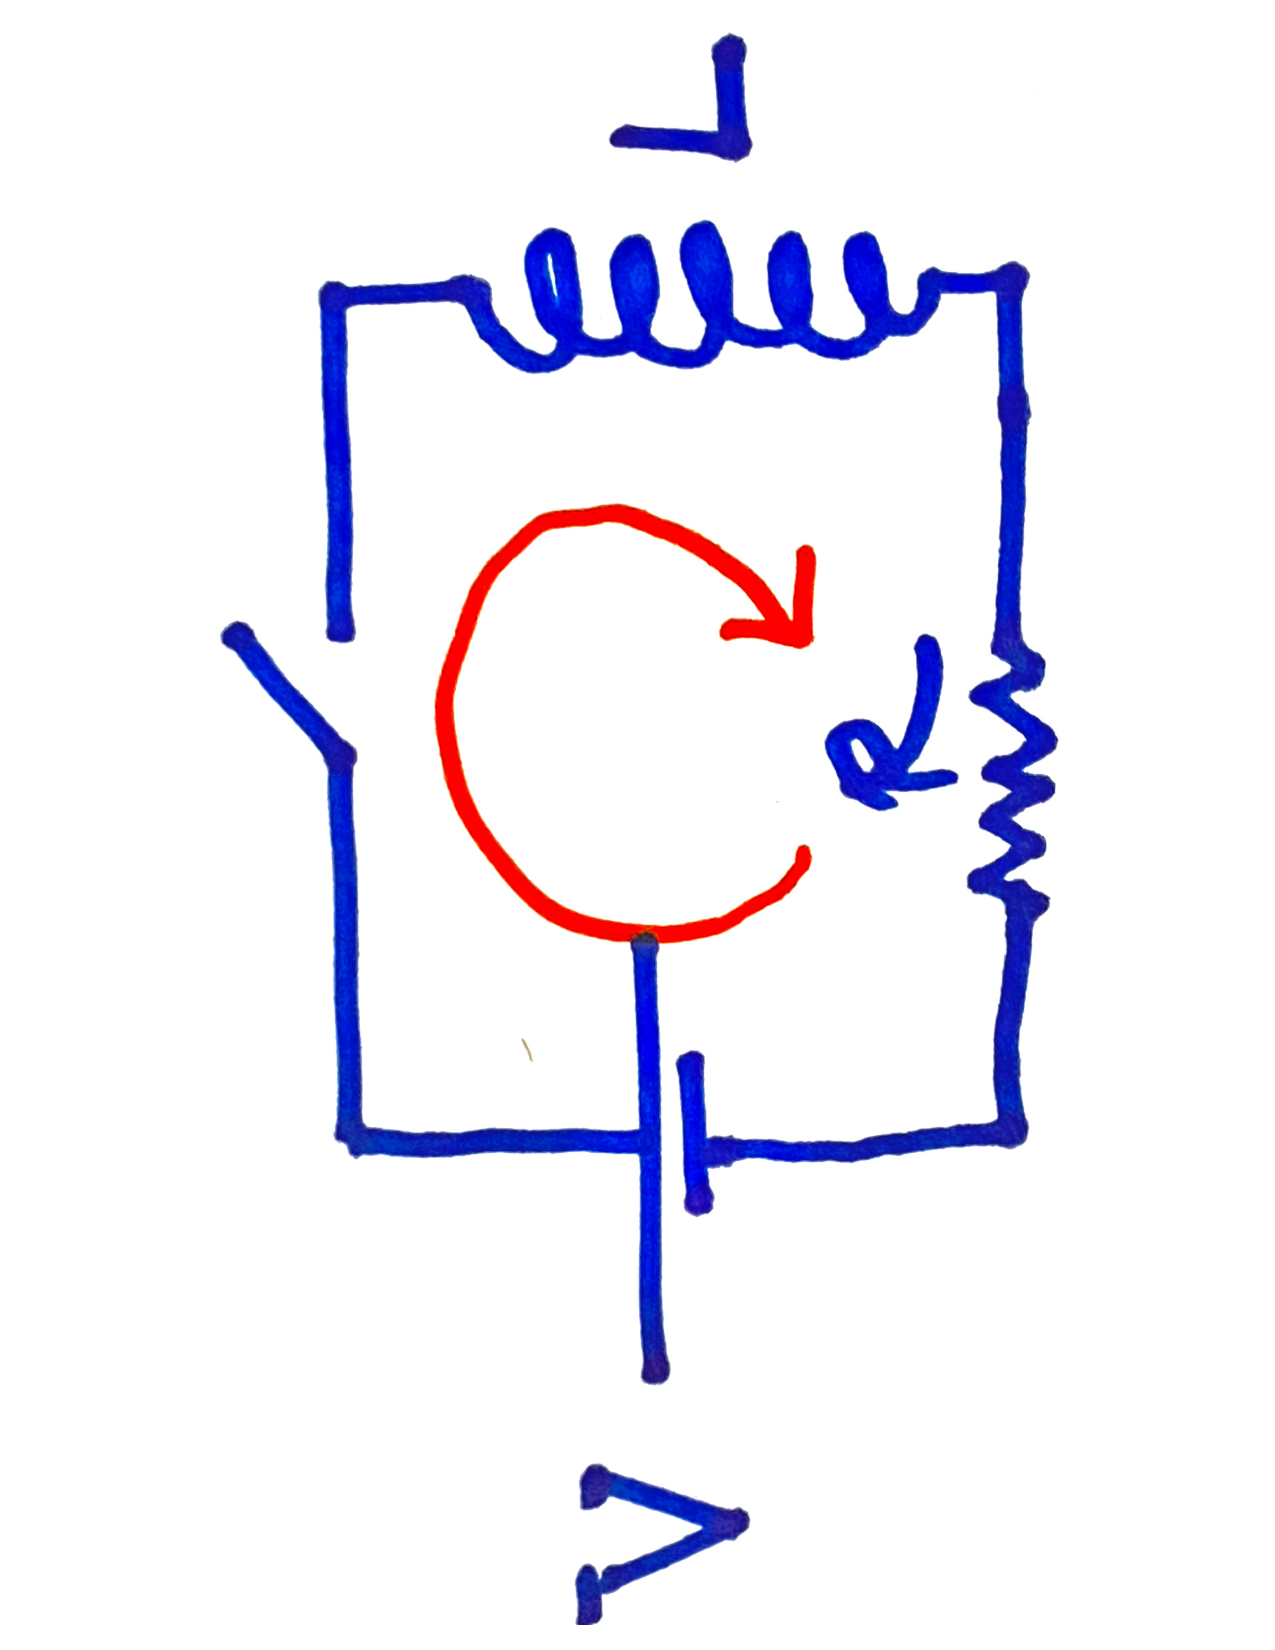
\includegraphics[width=\marginparwidth]{VLRcircuit.pdf}}

\startproblem%
You have a rigid rectangular
conducting loop of width $w$ (in the $y$ direction) and length $\ell$
(in the $x$ direction) being pulled in the $x$ direction at speed
$v$. The loop is partially in a region of magnetic field, and
partially out; it is being pulled into the field. In
the region that has magnetic field, the field has magnitude $B$
pointing in the $z$ direction. What is the current $I$ induced in this
loop? Assume the loop has total resistance $R$.
What is the force $F$ with which the loop has to be pulled, given this induced current?

\end{document}
